\documentclass[unicode,12pt,a4paper,oneside,fleqn]{article}
\usepackage{styles/main} 
\ifpdf
    \hypersetup{
        pdffitwindow=false,
        pdfstartview={FitH},
        pdftitle={Курсовая работа за 5 курс},
        pdfauthor={Бедняков А.И.}
        pdfproducer={Бедняков А.И.},
        pdfsubject={Методы криптоанализа},
    }
\fi

\begin{document}
    \begin{titlepage}
    \begin{center}
        МИНОБРНАУКИ РОССИИ
        \linebreak

        \vspace{48pt}{
        Федеральное государственное бюджетное образовательное 
        учреждение высшего профессионального образования
        \linebreak
        «Ярославский государственный университет им. П.Г. Демидова»
        }
        \linebreak

        \vspace{1em}{
        Кафедра компьютерной безопасности и
        математических методов обработки информации
        }
    \end{center}

    \vspace{1em}

    \begin{center}
        \textsc{\textbf{Курсовая работа}}
        \linebreak
        \textsc{\textbf{«Реализация "взломов" криптографических методов»}}
    \end{center}

    \vspace{6em}

	\begin{flushright}
        Научный руководитель \\
        \rule{2,2cm}{1pt} Белова Л.Ю. \\
        «\rule{0,5cm}{1pt}» \rule{2,5cm}{1pt} 2013 г.

        \vspace{1.5em}

        Студент группы КБ-51 \\
        \rule{2cm}{1pt} Бедняков А.И. \\
        «\rule{0,5cm}{1pt}» \rule{2,5cm}{1pt} 2013 г.
	\end{flushright}

    \vspace{\fill}

    \begin{center}
        Ярославль 2013
    \end{center}
\end{titlepage}

    \begin{abstract}
Мы будем делать...
\end{abstract}


    \tableofcontents
    \pagebreak

    \section{Введение}
    <kjrb


    \pagebreak
    
    \section{Лингвистический и статистический анализ}
    <kjrb


    \subsection{Словарный перебор}

Наиболее простой метод --- сравнение всех слов текста со словарем 
корректных слов нужного языка. Полученное количество совпавших слов
делится на количество слов исследуемого текста. Результирующая 
величина может рассматриваться как вероятность того, что данный 
текст принадлежит рассматриваемому языку.

Подобная оценка подходит целям данной работы --- критерий по 
этой 'вероятности' позволит отделить зерна от плевел и выделить 
наиболее пригодный вариант --- ложное срабатывание в общем случае 
маловероятно из-за специфики процесса. При негативном результате мы видим 
несвязный набор символов.

\begin{listing}[1]{1}
In [1]: import linguistics
In [2]: a = open('../sample/warandpeace', 'r').readlines()
In [3]: linguistics.istext_dict(a)
('ru', 0,864536523576)
\end{listing}

Здесь в первой строке подключается лингвистический модуль, 
во второй строке тестируемый текст записывается в переменную
$a$, и наконец в третьей вызывается метод определения языка 
по словарю. Метод возвращает предполагаемый язык и 
величину соответствия $V = \frac{n}{N}$, где $n$ --- количество
совпавших слов, а $N$ --- количество слов в тексте.

Практика демонстрирует жизнеспособность такого метода. Во-первых, 
составление 
словаря для известного языка в необходимой стилистике не представляет 
трудности при условии доступности интернета. Во-вторых, современные 
компьютерные мощности позволяют сравнительно быстрое выполнение 
подобного анализа:

\begin{listing}[1]{1}
# /usr/bin/time python ./cipher/linguistics.py -d ./sample/warandpeace 
python  710.10s user 780.55s system 0% cpu 20.002 total
\end{listing}

Здесь мы вызываем метод $istext\_dict$ через внешний 
интерфейс и отслеживаем время выполнения команды с помощью 
стандартной утилиты UNIX time.

Возможно совершествование данного метода путем написания более 
эффективных структур для хранения словаря, грамотной сериализации и 
использования оптимизированных алгоримов поиска по сортированному 
массиву. Но, как будет показано, в этом нет необходимости.
Во-первых мы не перешагнем известное ограничение сложности в 
$O(log(n))$ для алгоритмов поиска. Во-вторых, отсустствует необходимость 
в строгом соответствии текста языку определенному в словаре.
В-третьих, текст шифрограммы сравнительно редко содержит
пробелы, либо им нельзя доверять.

    \subsection{Использование n-грамм}
Второй метод анализа так же основан на работе со словарем, 
но обладает рядом преимуществ.

\DEF\textit{n-грамма} — последовательность из n элементов. С 
семантической точки зрения, это может быть последовательность 
звуков, слогов, слов или букв. На практике чаще встречается 
n-грамма как ряд слов. Последовательность из двух последовательных 
элементов часто называют биграммы, последовательность из трех 
элементов называется триграмма. Не менее четырех и выше элементов 
обозначаются как n-грамма, n заменяется на количество последовательных 
элементов.

В области обработки естественного языка, n-граммы используется 
в основном для предугадывания на основе вероятностных моделей. 
n-граммная модель рассчитывает вероятность последнего слова 
n-граммы, если известны все предыдущие. При использовании этого 
подхода для моделирования языка предполагается, что появление 
каждого слова зависит только от предыдущих слов.

\DEF\textit{Инвертированный индекс} — структура данных, в которой 
для каждого слова коллекции документов в соответствующем списке 
перечислены все места в коллекции, в которых оно встретилось. 
Инвертированный индекс используется для поиска по текстам.

Опишем как решается задача нахождения документов в которых встречаются 
все слова из поискового запроса. При обработке однословного поискового 
запроса, ответ уже есть в инвертированном индексе — достаточно 
взять список соответствующий слову из запроса. При обработке 
многословного запроса берутся списки, соответствующие каждому 
из слов запроса и пересекаются.

Пусть у нас есть корпус из трех текстов $T_0$='it is what it is', 
$T_1$='what is it' и $T_2$='it is a banana', тогда инвертированный 
индекс будет выглядеть следующим образом:

\begin{verbatim}
"a":      {2}
"banana": {2}
"is":     {0, 1, 2}
"it":     {0, 1, 2}
"what":   {0, 1}
\end{verbatim}

Здесь цифры обозначают номера текстов, в которых встретилось 
соответствующее слово. Тогда отработка поискового 'what is it
' запроса даст следующий результат $\{0,1\} \cap \{0,1,2\} \cap 
\{0,1,2\} = \{0,1\}$.

\begin{listing}[1]{1}
In [1]: import linguistics
In [2]: a = open('../sample/warandpeace', 'r').readlines()
In [3]: linguistics.istext\_wgramms(a)
0,892340923846
\end{listing}

Время исполнения теста так-же в разы превышает результат 
перебора по словарю:

\begin{listing}[1]{1}
# /usr/bin/time python ./cipher/linguistics.py -w ./sample/warandpeace 
python  210.10s user 280.55s system 0% cpu 20.002 total
\end{listing}

Такой метод, как и словарный перебор не справляется с 
текстом, в котором отсутствуют пробелы. Для решения 
этой проблемы необходимо сделать атомарным элементом 
не слова в тексте, а букву. 

В фреймворке реализован метод поочередного теста текста с 
тетраграммами, триграммами и биграммами. Как только какой-либо 
из тестов получает ответ с велечиной $V$ выше некоторого порога 
(например в 0,8), этот результат возвращается в качестве 
ответа. Такой порядок тестов обусловлен характеристиками 
реализованного лексера. Вызов выглядит так-же как и 
в прошлом примере: 

\begin{listing}[1]{1}
In [1]: import linguistics
In [2]: a = open('../sample/warandpeace', 'r').readlines()
In [3]: linguistics.istext\_lgramms(a)
0,802304958733
\end{listing}

Время исполнения теста:

\begin{listing}[1]{1}
# /usr/bin/time python ./cipher/linguistics.py -l ./sample/warandpeace 
python  170.10s user 170.55s system 0% cpu 20.002 total
\end{listing}

Итак, метод буквенных n-грамм является наиболее эффективным
из рассмотренных и будет использоваться в фреймворке.

    \subsection{Индекс совпадений}

Рассмотрим текст, написанный на некотором языке. Алфавит данного языка будем полагать состоящим из $m$ букв. Рассмотрим достаточно длинную строку $\vec x$ из $n$ букв. Если $f_i$ задаёт количество $i$-той буквы алфавита в строке $\vec x$, то можно определить индекс совпадений как вероятность совпадения двух произвольных букв в строке:

    $$I \left( \vec x \right) = \sum\limits_i {f_i \frac{{f_i - 1}}{{n\left( {n - 1} \right)}}}$$

откуда при достаточно больших $n$ и определении $p_i$ как $p_i = f_i / n$ получаем приближённую формулу:

    $$I \left( \vec x \right) = \sum\limits_i p_i^2$$ 

    \subsection{Критерий $\chi^2$ (хи-квадрат)}

\DEF\textit{Критерий $\chi^2$ (хи-квадрат)}, или критерий Пирсона — наиболее часто употребляемый критерий для проверки гипотезы о законе распределения.

Для проверки критерия вводится статистика:

    $$\chi^2 = N\sum \frac{\left( P_i^{\mathrm{emp}} - P_i^{\mathrm{H_{0}}} \right)^2}{P_i^{\mathrm{H_{0}}}},$$

где $P_i^{\mathrm{H_{0}}} = F(x_i) - F(x_{i-1})$ — предполагаемая вероятность попадания в $i$-й интервал, $P_i^{\mathrm{emp}} = \frac{n_i}{N}$ — соответствующее эмпирическое значение, ${n_i}$ — число элементов выборки из $i$-го интервала, $N$ — полный объём выборки. Также используется расчет критерия по частоте, тогда:

    $$\chi^2 = \sum \frac{\left( V_i^{\mathrm{}} - NP_i^{\mathrm{H_{0}}} \right)^2}{NP_i^{\mathrm{H_{0}}}},$$

где $V_i$ — частота попадания значений в интервал. Эта величина, в свою очередь, является случайной (в силу случайности $\chi$) и должна подчиняться распределению $\chi^2$.

    \subsection{Реализация}
Написан подключаемый модуль $linguistics$, выполняющий все операции, 
связанные с естественными языками. Статистический анализ
содержится в базовом классе и будет описан далее.
Модуль состоит из 6 функций:

\begin{enumerate}
\item $get\_alphabet(lang)$ — возвращает алфавит с частотой встречамости 
    букв и некоторыми дополнительными характеристиками языка.
\item $define\_language(text)$ — определяет язык текста.
\item $istext\_dictionary(text)$ — словарный анализ.
\item $istext\_lgramms(text)$ — анализ n-грамм из слов.
\item $istext\_wgramms(text)$ — анализ n-грамм из букв.
\end{enumerate}

    \pagebreak

    \section{Классические шифры}
    <kjrb


    \subsection{Шифр Цезаря}

Шифр Цезаря — это вид шифра подстановки, в котором каждый символ 
в открытом тексте заменяется буквой находящейся на некоторое 
постоянное число позиций левее или правее него в алфавите.

Шифр назван в честь римского императора Гая Юлия Цезаря, использовавшего 
его для секретной переписки со своими генералами.

\subsubsection{Описание}

Если сопоставить каждому символу алфавита его порядковый номер 
(нумеруя с 0), то шифрование и дешифрование можно выразить формулами 
модульной арифметики:

    $$y=(x+k)\ \mod\ n$$
    $$x=(y-k+n)\ \mod\ n,$$

где $x$ — символ открытого текста, $y$ — символ шифрованного 
текста, $n$ — мощность алфавита, а $k$ — ключ.

\subsubsection{Криптоанализ, реализация простого перебора и архитектура базового класса}

Шифр Цезаря может быть легко взломан даже в случае, когда взломщик 
знает только зашифрованный текст. Можно рассмотреть две ситуации:

\begin{enumerate}
\item Известно что использовался простой шифр подстановки, но 
    не известно, что это — схема Цезаря;
\item Известно что использовался шифр Цезаря, но не известно 
   значение сдвига.
\end{enumerate}

В первом случае шифр может быть взломан, используя те же самые 
методы что и для простого шифра подстановки — частотный 
анализ с перебором по описанным ранее лингвистическим метрикам.
Таким образом, взломщик, вероятно, быстро 
заметит регулярность в решении и поймёт, что используемый шифр — 
это шифр Цезаря.

Во втором случае, взлом шифра является даже более простым. Существует 
не так много вариантов значений сдвига (26 для английского языка), 
все они могут быть проверены методом перебора.

Для обычного текста на естественном языке, скорее всего, будет 
только один вариант декодирования. Но, если использовать очень 
короткие сообщения, то возможны случаи, когда возможны несколько 
вариантов расшифровки с различными сдвигами. Например зашифрованный 
текст MPQY может быть расшифрован как «aden» так и как «know» 
(предполагая, что открытый текст написан на английском языке). 
Точно также «ALIIP» можно расшифровать как «dolls» или как «wheel
»; «AFCCP» как «jolly» или как «cheer».

Благодаря малому количеству ключей криптоанализ сводится
к применению функции расшифрования ко всем текстам и 
поиск в результатах текста с максимальной метрикой: 

\begin{listing}[1]{1}
import cipher.cesar
def dechiper(ctext):
    c = cipher.cesar(ctext)
    scores = [(fitness.score(c.decrypt(i)), i) for i in range(26)]
    return max(scores)
\end{listing}

Относитьельно шифра Цезаря осталось добавить, что
многократное шифрование никак не улучшает стойкость, так как 
применение шифров со сдвигом $a$ и $b$ эквивалентно применению шифра 
со сдвигом $a+b$. В математических терминах шифрование с различными 
ключами образует группу.

Прешло время обсудить реализацию каждого класса в фреймворке 

\begin{figure}[h]
\noindent\centering{
    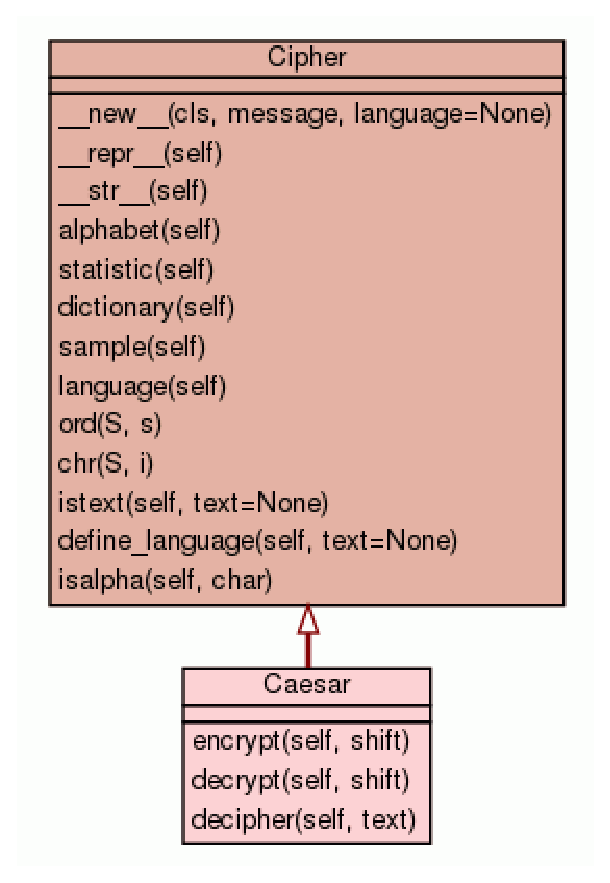
\includegraphics[width=65mm]{\globalImages/uml_cesar.eps}
}
\caption{UML диаграмма класса анализа шифра Цезаря}
\label{figUCesar}
\end{figure}


\begin{figure}[h]
\noindent\centering{
    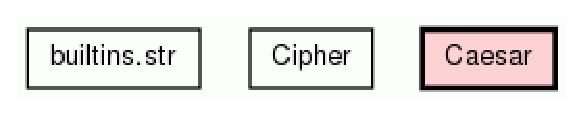
\includegraphics[width=75mm]{\globalImages/hierarchy_caesar.eps}
}
\caption{Иерархическая диаграмма класса анализа шифра Цезаря}
\label{figICesar}
\end{figure}


\begin{figure}[h]
\noindent\centering{
    
\includegraphics[width=65mm]{\globalImages/uml_cached.eps}
}
\caption{UML диаграмма класса для кеширования свойств}
\label{figCached}
\end{figure}

    \subsection{Аффинный шифр}

Аффинный шифр — это частный случай более общего моноалфавитного шифра 
подстановки. К шифрам подстановки относятся также шифр Цезаря, 
ROT13 и Атбаш. Поскольку аффинный шифр легко дешифровать, 
он обладает слабыми криптографическими свойствами.

\subsubsection{Описание}

В аффинном шифре каждой букве алфавита размера m ставится в 
соответствие число из диапазона $[0, ..., m - 1]$. 
Затем при помощи модульной арифметики для каждого числа, соответствующего 
букве исходного алфавита, вычисляется новое число, которое заменит 
старое в шифротексте. Функция шифрования для каждой буквы

    $$\mbox{E}(x) = (ax + b) \mod{m},$$

где модуль $m$ — размер алфавита, а пара $a$ и $b$ — ключ шифра. Значение 
$a$ должно быть выбрано таким, что $a$ и $m$ — взаимно простые числа. Функция 
расшифрования

    $$\mbox{D}(x) = a^{-1} \times (x - b) \mod{m},$$

где $a^{-1}$ — обратное к $a$ число по модулю $m$. То есть оно удовлетворяет 
уравнению

    $$1 \equiv a \times a^{-1} \mod{m}.$$

Обратное к $a$ число существует только в том случае, когда $a$ и $m$ — взаимно 
простые. Значит, при отсутствии ограничений на выбор числа $a$ расшифрование 
может оказаться невозможным. Покажем, что функция расшифрования является 
обратной к функции шифрования:

\begin{equation}
    \begin{matrix}
        \mbox{D}(\mbox{E}(x)) 
          &= &a^{-1} \times (\mbox{E}(x) - b) \mod{m} \\ 
          &= &a^{-1} \times ((ax + b) - b) \mod{m} \\ 
          &= &a^{-1} \times (ax + b - b) \mod{m} \\ 
          &= &a^{-1} \times ax \mod{m}\\ 
          &= &x \mod{m}. 
    \end{matrix}
\end{equation}

Количество возможных ключей для аффинного шифра можно записать 
с помощью функции Эйлера как $\varphi(m) \times m$.

\subsubsection{Криптоанализ}

Так как аффинный шифр является по сути моноалфавитным шифром замены
, то он обладает всеми уязвимостями этого класса шифров. Шифр Цезаря —
это аффинный шифр с $a = 1$, что сводит функцию шифрования к простому 
линейному сдвигу.

В случае шифрования сообщений на русском языке (т. е. с помощью $m = 33$) 
существует 627 нетривиальных аффинных шифров, не учитывая 33 тривиальных шифра 
Цезаря. Это число легко посчитать, зная, что существует всего 20 чисел 
взаимно простых с 33 и меньших 33 (а это и есть возможные значения 
$a$). Каждому значению a могут соответствовать 33 разных дополнительных 
сдвига (значение $b$); то есть всего существует 2033 или 660 возможных 
ключей. Аналогично, для сообщений на английском языке (т.е. $m = 26$) 
всего существует 1226 или 312 возможных ключей. Такое ограниченное 
количество ключей приводит к тому, что система крайне не криптостойка 
с точки зрения принципа Керкгоффса.

Основная уязвимость шифра заключается в том, что криптоаналитик может 
выяснить (путем частотного анализа, полного перебора, угадывания или 
каким-либо другим способом) соответствие между двумя любыми буквами 
исходного текста и шифротекста. Тогда ключ может быть найдет путем 
решения системы уравнений. Кроме того, так мы знаем, что $a$ и $m$ — взаимно 
простые, это позволяет уменьшить количество проверяемых ключей для 
полного перебора.

Преобразование, подобное аффинному шифру, используется в линейном 
конгруэнтном методе (разновидности генератора псевдослучайных чисел).
Этот метод не является криптостойким по той же причине, что и аффинный 
шифр.


    \subsection{Шифр Виженера}
Шифр Виженера (фр. Chiffre de Vigenère) — метод полиалфавитного 
шифрования буквенного текста с использованием ключевого слова.

Этот метод является простой формой многоалфавитной замены. Шифр 
Виженера изобретался многократно. Впервые этот метод описал Джован 
Баттиста Беллазо (итал. Giovan Battista Bellaso) в книге La cifra 
del. Sig. Giovan Battista Bellasо в 1553 году, однако в XIX веке 
получил имя Блеза Виженера, французского дипломата. Метод прост 
для понимания и реализации, он является недоступным для простых 
методов криптоанализа.

Первое точное документированное описание многоалфавитного шифра 
было сформулированно Леоном Баттиста Альберти в 1467 году, для 
переключения между алфавитами использовался металлический шифровальный 
диск. Система Альберти переключает алфавиты после нескольких 
зашифрованных слов. Позднее, в 1518 году, Иоганн Трисемус в своей 
работе «Полиграфия» изобрел tabula recta — центральный компонент 
шифра Виженера.

То, что сейчас известно под шифром Виженера, впервые описал Джованни 
Батиста Беллазо в своей книге La cifra del. Sig. Giovan Battista 
Bellasо. Он использовал идею tabula recta Трисемуса, но добавил 
ключ для переключения алфавитов шифра через каждую букву.

Блез Виженер представил свое описание простого, но стойкого шифра 
перед комиссией Генриха III во Франции в 1586 году, и позднее 
изобретение шифра было присвоено именно ему. Давид Кан в своей 
книге «Взломщики кодов» отозвался об этом осуждающе, написав, 
что история «проигнорировала важный факт и назвала шифр именем 
Виженера, несмотря на то, что он ничего не сделал для его создания».

Шифр Виженера имел репутацию исключительно стойкого к «ручному
» взлому. Известный писатель и математик Чарльз Лютвидж Доджсон 
(Льюис Кэрролл) назвал шифр Виженера невзламываемым в своей статье 
«Алфавитный шифр» англ. The Alphabet Cipher, опубликованной в 
детском журнале в 1868 году. В 1917 году Scientific American 
также отозвался о шифре Виженера, как о неподдающемся взлому. 
Это представление было опровергнуто после того, как Касиски полностью 
взломал шифр в XIX веке, хотя известны случаи взлома этого шифра 
некоторыми опытными криптоаналитиками еще в XVI веке.

Шифр Виженера достаточно прост для использования в полевых условиях
, особенно если применяются шифровальные диски. Например, «конфедераты
» использовали медный шифровальный диск для шифра Виженера в 
ходе Гражданской войны. Послания Конфедерации были далеки от 
секретных, и их противники регулярно взламывали сообщения. Во 
время войны командование Конфедерации полагалось на три ключевых 
словосочетания: «Manchester Bluff», «Complete Victory» и — так 
как война подходила к концу — «Come Retribution».

Гилберт Вернам попытался улучшить взломанный шифр (он получил 
название шифр Вернама-Виженера в 1918 году), но, несмотря на 
его усовершенствования, шифр так и остался уязвимым к криптоанализу
. Однако работа Вернама в конечном итоге все же привела к получению 
шифра, который действительно невозможно взломать.

\subsubsection{Описание}

В шифре Цезаря каждая буква алфавита сдвигается на несколько 
строк; например в шифре Цезаря при сдвиге +3, A стало бы D, B 
стало бы E и так далее. Шифр Виженера состоит из последовательности 
нескольких шифров Цезаря с различными значениями сдвига. Для 
зашифровывания может использоваться таблица алфавитов, называемая 
tabula recta или квадрат (таблица) Виженера. Применительно к 
латинскому алфавиту таблица Виженера составляется из строк по 
26 символов, причём каждая следующая строка сдвигается на несколько 
позиций. Таким образом, в таблице получается 26 различных шифров 
Цезаря. На разных этапах кодировки шифр Виженера использует различные 
алфавиты из этой таблицы. На каждом этапе шифрования используются 
различные алфавиты, выбираемые в зависимости от символа ключевого 
слова. Например, предположим, что исходный текст имеет вид:

ATTACKATDAWN

Человек, посылающий сообщение, записывает ключевое слово («LEMON») 
циклически до тех пор, пока его длина не будет соответствовать 
длине исходного текста:

LEMONLEMONLE

Первый символ исходного текста A зашифрован последовательностью 
L, которая является первым символом ключа. Первый символ L шифрованного 
текста находится на пересечении строки L и столбца A в таблице 
Виженера. Точно так же для второго символа исходного текста используется 
второй символ ключа; то есть второй символ шифрованного текста 
X получается на пересечении строки E и столбца T. Остальная часть 
исходного текста шифруется подобным способом.

Исходный текст:      ATTACKATDAWN
Ключ:                LEMONLEMONLE
Зашифрованный текст: LXFOPVEFRNHR

Расшифровывание производится следующим образом: находим в таблице 
Виженера строку, соответствующую первому символу ключевого слова
; в данной строке находим первый символ зашифрованного текста
. Столбец, в котором находится данный символ, соответствует первому 
символу исходного текста. Следующие символы зашифрованного текста 
расшифровываются подобным образом.

Если буквы A-Z соответствуют числам 0-25, то шифрование и расшифрование Виженера 
можно записать в виде формул:

    $$C_i \equiv (P_i + K_i) \mod\ 26$$
    $$P_i \equiv (C_i - K_i + 26) \mod\ 26$$

\subsubsection{Криптоанализ, работа с полиалфавитными шифрами}

Шифр Виженера «размывает» характеристики частот появления символов 
в тексте, но некоторые особенности появления символов в тексте 
остаются. Главный недостаток шифра Виженера состоит в том, что 
его ключ повторяется. Поэтому простой криптоанализ шифра может 
быть построен в два этапа:

Поиск длины ключа. Можно анализировать распределение частот в 
зашифрованном тексте с различным прореживанием. То есть брать 
текст, включающий каждую 2-ю букву зашифрованного текста, потом 
каждую 3-ю и т. д. Как только распределение частот букв будет 
сильно отличаться от равномерного (например, по энтропии), то 
можно говорить о найденной длине ключа.

\paragraph{Метод Касиски}

В 1863 году Фридрих Касиски был первым, кто опубликовал успешный 
алгоритм атаки на шифр Виженера, хотя Чарльз Беббидж разработал 
этот алгоритм уже в 1854 году. В то время когда Беббидж занимался 
взломом шифра Виженера, John Hall Brock Thwaites представил новый 
шифр в «Journal of the Society of the Arts»; когда Беббидж показал
, что шифр Thwaites’а является лишь частным случаем шифра Виженера
, Thwaites предложил ему его взломать. Беббидж расшифровал текст
, который оказался поэмой «The Vision of Sin» Альфреда Теннисона
, зашифрованной ключевым словом Emily — именем жены поэта.

Тест Касиски опирается на то, что некоторые слова, такие как 
«the» могут быть зашифрованы одинаковыми символами, что приводит 
к повторению групп символов в зашифрованном тексте. Например: 
сообщение, зашифрованное ключом ABCDEF , не всегда одинаково 
зашифрует слово «crypto».

Зашифрованный текст в данном случае не будет повторять последовательности 
символов, которые соответствуют повторным последовательностям 
исходного текста. В данном шифрованном тексте есть несколько 
повторяющихся сегментов, которые позволяют криптоаналитику найти 
длину ключа.

Более длинные сообщения делают тест более точным, так как они 
включают в себя больше повторяющихся сегментов зашифрованного 
текста. В данном шифрованном тексте есть несколько повторяющихся 
сегментов, которые позволяют криптоаналитику найти длину ключа.

Расстояние между повторяющимися DYDUXRMH равно 18, это позволяет 
сделать вывод, что длина ключа равна одному из значений: 18,9
,6,3 или 2. Расстояние между повторяющимися NQD равно 20. Из 
этого следует, что длина ключа равна 20 или 10, или 5, или 4 
или 2. Сравнивая возможные длины ключей, можно сделать вывод, 
что длина ключа (почти наверняка) равна 2.

\paragraph{Тест Фридмана}

(иногда называемый каппа-тест) был изобретен Вильямом 
Фридманом в 1920 году. Фридман использовал индекс совпадения, 
который измеряет частоты повторения символов, чтобы взломать 
шифр. Зная вероятность $\kappa_p$ того, что два случайно выбранных 
символа текста совпадают (примерно 0,067 для англ. языка) и вероятность 
совпадения двух случайно выбранных символов алфавита $\kappa_r$ 
(примерно 1 / 26 = 0,0385 для англ. языка), можно оценить длину 
ключа как:

    $${\kappa_p-\kappa_r}\over{\kappa_o-\kappa_r}$$

Из наблюдения за частотой совпадения следует:

    $$\kappa_o=\frac{\sum_{i=1}^{c}n_i(n_i -1)}{N(N-1)}$$

Где $С$ — размер алфавита (26 символов для англ. языка), $N$ — длина 
текста, и $n_1$ до $n_c$ — наблюдаемые частоты повторения символов 
зашифрованного текста. Однако, это только приблизительное значение
, точность которого увеличивается при большем размере текста. 
На практике это было бы необходимо для перебора различных ключей 
приближаясь к исходному.

\paragraph{Частотный анализ}

Как только длина ключа становится известной, зашифрованный текст 
можно записать во множество столбцов, каждый из которых соответствует 
одному символу ключа. Каждый столбец состоит из исходного текста
, который зашифрован шифром Цезаря; ключ к шифру Цезаря является 
всего-навсего одним символом ключа для шифра Виженера, который 
используется в этом столбце. Используя методы, подобные методам 
взлома шифра Цезаря, можно расшифровать зашифрованный текст. 
Усовершенствование теста Касиски, известное как метод Кирхгофа
, заключается в сравнении частоты появления символов в столбцах 
с частотой появления символов в исходном тексте для нахождения 
ключевого символа для этого столбца. Когда все символы ключа 
известны, криптоаналитик может легко расшифровать шифрованный 
текст, получив исходный текст. Метод Кирхгофа не применим, когда 
таблица Виженера скремблирована, вместо использования обычной 
алфавитной последовательности, хотя тест Касиски и тесты совпадения 
всё ещё могут использоваться для определения длины ключа для 
этого случая.

    \subsection{Энигма}
Энигма — портативная шифровальная машина, использовавшаяся для шифрования 
и дешифрования секретных сообщений. Более точно, Энигма — целое семейство 
электромеханических роторных машин, применявшихся с 20-х годов XX 
века.

Энигма использовалась в коммерческих целях, а также в военных и государственных 
службах во многих странах мира, но наибольшее распространение получила 
в нацистской Германии во время Второй мировой войны — именно Энигма 
вермахта (Wehrmacht Enigma) — германская военная модель — чаще всего 
является предметом дискуссий.

\subsubsection{Описание}
Как и другие роторные машины, Энигма состояла из комбинации механических 
и электрических подсистем. Механическая часть включала в себя клавиатуру
, набор вращающихся дисков — роторов, — которые были расположены вдоль 
вала и прилегали к нему, и ступенчатого механизма, двигающего один 
или несколько роторов при каждом нажатии на клавишу.

Конкретный механизм работы мог быть разным, но общий принцип был таков
: при каждом нажатии на клавишу самый правый ротор сдвигается на одну 
позицию, а при определённых условиях сдвигаются и другие роторы. Движение 
роторов приводит к различным криптографическим преобразованиям при 
каждом следующем нажатии на клавишу на клавиатуре.

Механические части двигались, замыкая контакты и образуя меняющийся 
электрический контур (то есть, фактически, сам процесс шифрования 
букв реализовывался электрически). При нажатии на клавишу клавиатуры 
контур замыкался, ток проходил через различные цепи и в результате 
включал одну из набора лампочек, и отображавшую искомую букву кода
. (Например: при шифровке сообщения, начинающегося с ANX…, оператор 
вначале нажимал на клавишу A — загоралась лампочка Z — то есть Z и 
становилась первой буквой криптограммы. Далее оператор нажимал N и 
продолжал шифрование таким же образом далее).

Таким образом, постоянное изменение электрической цепи, через которую 
шёл ток, вследствие вращения роторов позволяло реализовать многоалфавитный 
шифр подстановки, что давало высокую, для того времени, устойчивость шифра.

Роторы — сердце Энигмы. Каждый ротор представлял собой диск примерно 
10 см в диаметре, сделанный из эбонита или бакелита, с пружинными 
штыревыми контактами на одной стороне ротора, расположенными по окружности
. На другой стороне находилось соответствующее количество плоских 
электрических контактов. Штыревые и плоские контакты соответствовали 
буквам в алфавите (обычно это были 26 букв от A до Z). При соприкосновении 
контакты соседних роторов замыкали электрическую цепь. Внутри ротора 
каждый штыревой контакт был соединён с одним из плоских. Порядок соединения 
мог быть различным.

Сам по себе ротор производил очень простой тип шифрования: элементарный 
шифр замены. Например, контакт, отвечающий за букву E, мог быть соединён 
с контактом буквы T на другой стороне ротора. Но при использовании 
нескольких роторов в связке (обычно трёх или четырёх) за счёт их постоянного 
движения получается более надёжный шифр.

Преобразование Энигмы для каждой буквы может быть определено математически 
как результат перестановок. Рассмотрим трёхроторную армейскую модель
. Положим, что P обозначает коммутационную панель, U обозначает отражатель
, а L, M, R обозначают действия левых, средних и правых роторов соответственно
. Тогда шифрование E может быть выражено как:

    $$E = PRMLUL^{-1}M^{-1}R^{-1}P^{-1}$$

После каждого нажатия клавиш ротор движется, изменяя трансформацию
. Например, если правый ротор R проворачивается на i позиций, происходит 
трансформация $\rho^iR\rho^{-i}$, где ρ — циклическая перестановка
, проходящая от A к B, от B к C, и так далее. Таким же образом, средний 
и левый ротор могут быть обозначены как j и k вращений M и L. Функция 
шифрования в этом случае может быть отображена следующим образом:

    $$E = P(\rho^iR\rho^{-i})(\rho^{j}M\rho^{-j})(\rho^{k}L\rho^{-k})U(\rho^kL^{-1}\rho^{-k})(\rho^{j}M^{-1}\rho^{-j})(\rho^{i}R^{-1}\rho^{-i})P^{-1}$$

\subsubsection{Криптоанализ}
Попытки «взломать» Энигму не предавались гласности до конца 1970-х
. После этого интерес к Энигме значительно возрос, и множество шифровальных 
машин представлено к публичному обозрению в музеях США и Европы.

В Немецком музее в Мюнхене находятся оба немецких военных варианта 
трёх- и четырёхроторной Энигмы, есть и устаревшие гражданские модели
. Работающая модель представлена также в Международном шифровальном 
музее в Форт-Миде (Fort Meade), в Музее компьютерной истории (Computer 
History Museum) в США, в Блетчли-Парке (Bletchley Park) в Великобритании
, в Австралийском военном мемориале (Australian War Memorial) в Канберре
, а также в Германии, США, Великобритании и в некоторых других странах 
Европы.

В 2007 году запущен проект распределённых вычислений Enigma@Home, 
целью которого является взлом трех зашифрованных сообщений Энигмы, 
перехваченных в северной Атлантике в 1942 году.

    \pagebreak

    \section{Бинарные шифры}
    <kjrb


    \subsection{XOR}

XOR - это побитовое сложение по модулю (с инвертированием при переполнении), 
например, $1+1=0$ т.к. $1$ - максимальное значение. Все варианты:

$$0 \oplus 0=0$$
$$0 \oplus 1=1$$
$$1 \oplus 1=0$$

\subsubsection{Описание}
То есть, операция $z = x \oplus y$ по сути поразрядная (побитовая — 
результат не зависит от соседних битов). Если только один из 
соответствующих битов равен 1, то результат 1. А если оба 0 или 
оба 1, то результат 0. Если внимательно посмотреть на результат 
применения XOR к двум двоичным числам, то можно заметить, что 
мы можем восстановить одно из слагаемых при помощи второго: $x 
= z \oplus y$ или $y = z \oplus x$. 

\subsubsection{Криптоанализ}

Отсюда можно сделать следующие выводы: зная число y и применяя 
XOR к $x$, мы получим $z$. Затем, мы, опять же используя $y$, получим 
из $z$ обратно число $x$. Таким образом мы можем преобразовать последовательность 
чисел $(x)_i$ в последовательность $(z)_i$. Теперь мы можем назвать 
число y кодирующим (или шифрующим) ключом. Если человек не знает 
ключа, то он не сможет восстановить исходную последовательность 
чисел $(x)_i$.

Поскольку каждая буква будет представлена в шифротексте 
одним и тем же кодом $z$, то воспользуясь частотным словарем взломщик 
сможет вычислить шифрующий ключ $y$, если у него будет в распряжениии 
достаточно длинный шифротекст. 

В случае длинного ключа применяются уже разодранные методы 
анализа из шифра Виженера.


    \subsection{Blowfish}

Blowfish --- это алгоритм, разработанный Брюсом Шнайером специально 
для реализации на больших микропроцессорах. Алгоритм Blowfish 
не запатентован.

Алгоритм Blowfish оптимизирован для применения в системах, не 
практикующих частой смены ключей, например, в линиях связи и 
программах автоматического шифрования файлов. При реализации 
на 32-битовых микропроцессорах с большим размером кэша данных
, например, процессорах Pentium и PowerPC, алгоритм Blowfish 
заметно быстрее DES.

\subsubsection{Описание шифра Blowfish}

Blowfish представляет собой 64-битовый блочный алгоритм шифрования 
с ключом переменной длины. Алгоритм состоит из двух частей: расширения 
ключа и шифрования данных. Расширение ключа преобразует ключ 
длиной до 448 битов в несколько массивов подключей общим размером 4168 байт.

Шифрование данных заключается в последовательном исполнении простой 
функции 16 раз. На каждом раунде выполняются зависимая от ключа 
перестановка и зависимая от ключа и данных подстановка. Используются 
только операции сложения и XOR над 32-битовыми словами. Единственные 
дополнительные операции каждого раунда - четыре взятия данных 
из индексированного массива.
То есть, алгоритм Blowfish представляет собой сеть Фейстеля, состоящей 
из 16 раундов. На вход подается 64-битовый элемент данных $х$.

В алгоритме Blowfish используется множество подключей. Эти подключи 
должны быть вычислены до начала зашифрования или расшифрования данных.

Подключи рассчитываются с помощью самого алгоритма Blowfish. 
Вот какова точная последовательность действий:
\begin{enumerate}
\item Сначала Р-массив, а затем четыре S-блока по порядку инициализируются 
    фиксированной строкой.
\item Выполняется операция XOR над Р1 с первыми 32 битами ключа, 
    XOR над Р2 со вторыми 32 битами ключа, и т.д. для всех битов 
    ключа (вплоть до Р18). Операция XOR выполняется циклически над 
    битами ключа до тех пор, пока весь Р-массив не будет инициализирован.
\item Используя подключи, полученные на этапах 1 и 2, алгоритм 
    Blowfish шифрует строку из одних нулей.
\item Р1 и Р2 заменяются результатом этапа 3.
\item Результат этапа 3 шифруется с помощью алгоритма Blowfish 
    и модифицированных подключей.
\item Р3 и Р4 заменяются результатом этапа 5.
\item Далее по ходу процесса все элементы Р-массива, а затем 
    все четыре S-блока по порядку заменяются выходом постоянно меняющегося 
    алгоритма Blowfish.
\end{enumerate}

Всего для генерации всех необходимых подключей требуется 521 
итерация. Приложения могут сохранять подключи - нет необходимости 
выполнять процесс их получения многократно.
В реализациях Blowfish, в которых требуется очень высокая скорость,
цикл должен быть развернут, а все ключи храниться в кэше.

\subsubsection{Криптоанализ, обоснование стойкости}
Serge Vaudenay исследовал алгоритм Blowfish с известными 
$S$-блоками и $r$ раундами в работе \cite{vaudenay-blowfish}.
Дифференциальный криптоанализ может раскрыть 
$P$-массив с помощью $28^{r + 1}$ выбранных открытых текстов. Для 
некоторых слабых ключей, которые генерируют плохие $S$-блоки (вероятность 
выбора такого ключа составляет 1 к 214), это же вскрытие раскрывает 
$P$-массив с помощью всего $24^{r + 1}$. При неизвестных $S$-блоках это 
вскрытие может обнаружить использование слабого ключа, но не 
может определит сам ключ (ни $S$-блоки, ни $P$-массив). Это вскрытие 
эффективно только против вариантов с уменьшенным числом этапов 
и совершенно бесполезно против 16-этапного Blowfish.

Конечно, важно и раскрытие слабых ключей, даже хотя они скорее 
всего не будут использоваться. Слабым является ключ, для которого 
два элемента данного $S$-блока идентичны. До выполнения развертывания 
ключа невозможно определить, является ли он слабым. Если вы беспокоитесь 
об этом, вам придется выполнить развертывание ключа и проверить,
нет ли в $S$-одинаковых элементов. Хотя я не думаю, что это так 
уж необходимо.

Случаи успешного криптоанализа Blowfish не известны.

    \pagebreak

    \section{Определение алгоритма шифрования по шифротексту}
    Исследуемый сценарий --- исследуестя криптограмма и неизвестен
алгоритм шифрования, необходимо получить исходный открытый
текст.


    \pagebreak

    \section{Заключение}
    Во время написания курсовой работы мною были изучены классические
и блочные симметричные шифры на примере алгоритмов
шифр Цезаря, Афинный шифр, шифр Виженера, Xor, 
Enigma и Blowfish.

Передо мной стояла задача программной реализации программной 
реализации фреймворка для криптоанализа,
который имел бы удобный интерфейс пользователя и разработчика.

Эта задача была успешно выполнена. Фреймворк реализован, 
шифрует и расшифровывает файлы в соответствии с описаниями
изученных алгоритмов. В процессе написания мною были изучены некоторые 
тонкости программирования, связанные с шифрованием, а также с 
написанием программных интерфейсов.

Исходный код Python разработанного фреймворка и исходный 
код \TeX~курсовой работы доступны в Интернете в виде git 
репозитория по ссылке
\url{https://github.com/ch3sh1r/cryptanalysis}.

    %\section{Приложения}
%\begin{appendix}
    %\subsection{Исходный код}
        %\begin{enumerate}
            %\item{Функция верификации пароля}
            %\lstinputlisting{./code/motc-checker}
            %\item{Функция идентификации пользователя}
            %\lstinputlisting{./code/motc-id}
        %\end{enumerate}

    %\subsection{Блок-схема}
        %\includegraphics[width=160mm]{./img/atmel.png}
%\end{appendix}

%\pagebreak

    \addcontentsline{toc}{section}{Список литературы}
\begin{thebibliography}{1}
\bibitem{shna-pri} Шнайер Б., ``Прикладная криптография. Протоколы, алгоритмы, исходные тексты на языке Си'', 2002
\bibitem{shannon-inf} Шеннон К., «Работы по теории информации и кибернетике» (перевод В.Ф.Писаренко), 1963
\bibitem{fomi} Фомичев В.М. «Дискретная математика и криптология», М.: Диалог-МИФИ, 2003
\bibitem{yash} Ященко В.В. «Введение в криптографию», 1988
\bibitem{inte} Cryptography.ru. Статьи Интернет-сайтов. 
\end{thebibliography}

\end{document}
